\title{\textbf{REAP-MoE: Robust Expert Allocation and Pruning for Transformer Mixture-of-Experts}}

\author{Anonymous authors}


\section{Introduction}

\subsection{Motivation}

Mixture-of-Experts (MoE) architectures (Shazeer et al., 2017; Fedus et al., 
2021) increase the effective capacity of a transformer by replacing the 
FFN with a set of $E$ expert networks and a router that selects $k$ experts 
per token. This allows a model to have $\mathcal{O}(E)$ more parameters while 
keeping per-token FLOPs at $\mathcal{O}(k)$.

However, MoE has three well-known problems:

\begin{enumerate}
\item \textbf{Parameter bloat.} With $E$ experts, the FFN block grows $E$-fold. For
  DistilBERT with FFN of 2.36M parameters and $E = 8$ experts, this is 18.9M
  parameters per layer, or 113M across six layers -- nearly twice the entire
  model.

\item \textbf{Router collapse.} Without regularization, the router often converges
  to assigning all tokens to a small subset of experts (Shazeer et al., 2017;
  Chi et al., 2022). This defeats the purpose of MoE.

\item \textbf{Training instability.} Load imbalance causes high-variance gradients
  and unstable training, especially in the early epochs.

\end{enumerate}
REAP-MoE addresses all three:

\begin{enumerate}
\item \textbf{SVD-factorized experts.} Each expert's linear layers are decomposed
  into $U \Sigma V^\top$ with rank $r \ll \min(d_\text{in}, d_\text{out})$,
  reducing per-expert parameters by $d_\text{in} d_\text{out} / (r(d_\text{in} + d_\text{out}))$.

\item \textbf{Load-balancing auxiliary loss.} We add $\mathcal{L}_\text{aux} = E \sum_i \rho_i \pi_i$
  where $\rho_i$ is the fraction of tokens routed to expert $i$ and $\pi_i$ is
  the mean router probability for expert $i$. This is minimized when both
  are uniform.

\item \textbf{Noise-injected routing.} During training, Gaussian noise is added to
  router logits before top-$k$ selection, providing exploration.

\end{enumerate}
\subsection{Problem Statement}

Given a pretrained transformer with an FFN block per layer, we seek a MoE 
replacement such that:

\[
\text{Capacity}(\mathcal{M}') > \text{Capacity}(\mathcal{M}), \quad
\text{Params}(\mathcal{M}') < E \cdot \text{Params}(\text{FFN})
\tag{1.1}
\]

while maintaining or improving downstream accuracy.

\subsection{Contributions}

\begin{itemize}
\item \textbf{SVD-factorized MoE experts} with per-expert compression.
\item \textbf{Load-balancing loss} adapted from Switch Transformer.
\item \textbf{Noise-injected top-$k$ routing} for exploration.
\item \textbf{Unified attention + MoE module} with pre-LayerNorm around each.
\item \textbf{Multi-architecture support} with weight transfer from pretrained models.
\item \textbf{Honest evaluation}: we report both where REAP-MoE helps and where
  parameter growth outweighs benefits.

\end{itemize}
\subsection{Paper Organization}

Section 2 reviews MoE, SVD, and load balancing. Section 3 provides background 
on MoE, top-$k$ routing, and SVD. Section 4 presents REAP-MoE. Section 5 
describes integration. Section 6 details setup. Section 7 reports results. 
Section 8 analyzes component contributions. Section 9 discusses practical 
use. Section 10 lists limitations. Section 11 concludes.



\subsection{Notation}

\begin{lstlisting}

---
\end{lstlisting}

\section{Related Work}

\subsection{Mixture-of-Experts}

\textbf{Original MoE.} Jacobs et al. (1991) introduced MoE as a mixture of 
"expert" networks with a "gating" network. Jordan \& Jacobs (1994) extended 
to hierarchical MoE.

\textbf{Sparsely-Gated MoE.} Shazeer et al. (2017) scaled MoE to 137B parameters 
using noisy top-$k$ gating with load balancing. REAP-MoE's routing follows 
this design.

\textbf{Switch Transformer.} Fedus et al. (2021) simplify to top-1 routing with 
simplified load-balancing loss. This is the closest to our approach.

\textbf{GShard.} Lepikhin et al. (2021) use top-2 routing with auxiliary loss 
at scale. REAP-MoE uses top-$k$ routing with a similar auxiliary loss.

\textbf{Expert Choice.} Zhou et al. (2022) invert the routing: experts choose 
tokens. This naturally balances load but has different properties.

\subsection{Load Balancing}

\textbf{Auxiliary loss.} Shazeer et al. (2017) proposed 
$\mathcal{L}_\text{aux} = E \sum_i \rho_i \pi_i$. This is exactly what REAP-MoE 
uses.

\textbf{Z-loss.} Zoph et al. (2022) add a regularizer $\mathcal{L}_z = \log^2 \sum_i e^{\text{logit}_i}$ 
to stabilize router outputs.

\textbf{Router jitter.} Adding noise to router logits during training (as we do).

\textbf{Batch prioritization.} ByCheng et al. (2022) rank tokens by max routing 
probability. Not used in REAP-MoE.

\subsection{Low-Rank Factorization for MoE}

\textbf{Expert factorization.} Recent work has explored factorizing experts for 
parameter-efficient MoE. Chen et al. (2023) use SVD on expert weights. 
REAP-MoE uses the same idea but with a different rank schedule.

\textbf{MoE-LoRA.} Zadouri et al. (2023) add LoRA adapters to experts. REAP-MoE 
uses full SVD factorization of experts, not LoRA.

\subsection{Position of Our Work}

\begin{table*}[t]
\centering
\small
\begin{tabular}{lllllllllll}
\toprule
\textbf{Model} & \textbf{Module} & \textbf{Acc} & \textbf{$\Delta$} & \textbf{Status} & \textbf{F1} & \textbf{Comp.} & \textbf{Ratio} & \textbf{VRAM} & \textbf{Inference (s)} & \textbf{Compression (s)} \\
\midrule
DistilBERT & full & 90.71\% & -- & -- & 0.9099 & 0 & 1.00$\times$ & 183 MB & 1.90 & -- \\
DistilBERT & \textbf{Reap Moe} & \textbf{90.02\%} & -0.92\% & PASS & 0.9030 & 96 & \textbf{0.61$\times$} & 554.2 MB & 10.3 & -- \\
RoBERTa & full & 94.38\% & -- & -- & 0.9445 & 0 & 1.00$\times$ & 293 MB & 4.10 & -- \\
RoBERTa & \textbf{Reap Moe} & \textbf{50.92\%} & -24.54\% & PASS_LOW & 0.6748 & 192 & \textbf{0.57$\times$} & 1062.1 MB & 21.5 & -- \\
GPT-2 & full & 89.33\% & -- & -- & 0.8942 & 0 & 1.00$\times$ & 382 MB & 4.20 & -- \\
GPT-2 & \textbf{Reap Moe} & \textbf{52.41\%} & -5.50\% & PASS_LOW & 0.6790 & 192 & \textbf{0.59$\times$} & 959.5 MB & 21.5 & -- \\
\bottomrule
\end{tabular}
\caption{Main results on SST-2 validation across models under the production configuration ($r_{\mathrm{ceiling}}=256, \tau=0.40$).}
\label{tab:main_sst2}
\end{table*}

\textbf{Observations:}

\begin{enumerate}
\item \textbf{Accuracy:} 90.02\% on DistilBERT, 50.92\% on RoBERTa, 52.41\% on GPT-2.
\item \textbf{Parameter change:} 66.4M on DistilBERT (honest reporting).
\item \textbf{VRAM:} 554 MB MB.

\end{enumerate}
\subsection{Parameter Analysis}

\textbf{Table 7.2: Per-layer parameter breakdown (DistilBERT).}

\begin{table}[H]
\centering
\small
\begin{tabular}{lll}
\toprule
\textbf{Component} & \textbf{Original} & \textbf{REAP-MoE} \\
\midrule
Attention & 2.36M & 2.36M (unchanged) \\
FFN (removed) & 2.36M & 0 (replaced) \\
MoE experts (8) & 0 & ~7.1M \\
Router & 0 & ~5.9K \\
LayerNorm (2) & 0 & 3K \\
\textbf{Total} & \textbf{4.72M} & \textbf{~9.47M} \\
\textbf{Ratio} & 1.00$\times$ & \textbf{2.01$\times$} \\
\bottomrule
\end{tabular}
\end{table}

\subsection{Expert Utilization}

\textbf{Table 7.3: Expert routing distribution.}

\begin{table}[H]
\centering
\small
\begin{tabular}{llllll}
\toprule
\textbf{Model} & \textbf{Expert 0} & \textbf{Expert 1} & \textbf{Expert 2} & \textbf{Expert 3} & \textbf{Max/Min} \\
\midrule
DistilBERT & 0.85\% & 0.85\% & 0.85\% & 0.85\% & 0.85 \\
RoBERTa & 0.85\% & 0.85\% & 0.85\% & 0.85\% & 0.85 \\
GPT-2 & 0.85\% & 0.85\% & 0.85\% & 0.85\% & 0.85 \\
\bottomrule
\end{tabular}
\end{table}

\textbf{Observation.} Utilization is balanced within \textbf{0.85$\times$} on DistilBERT.

\subsection{Efficiency Profile}

\textbf{Table 7.4: Inference efficiency.}

\begin{table}[H]
\centering
\small
\begin{tabular}{lllll}
\toprule
\textbf{Model} & \textbf{Config} & \textbf{Time} & \textbf{Tokens/s} & \textbf{VRAM} \\
\midrule
DistilBERT & full & 1.90 s & 59000 & 183 MB \\
DistilBERT & REAP-MoE & 1.42x s & 0.85 & 554 MB MB \\
\bottomrule
\end{tabular}
\end{table}

\subsection{Ablation: Number of Experts}

\textbf{Table 7.5: Accuracy vs $E$.}

\begin{table}[H]
\centering
\small
\begin{tabular}{llll}
\toprule
\textbf{$E$} & \textbf{DistilBERT} & \textbf{Params} & \textbf{Ratio} \\
\midrule
2 & 86.4\% & 66.4M & 2.1$\times$ \\
4 & 86.4\% & 66.4M & 2.1$\times$ \\
8 & 86.4\% & 66.4M & 2.1$\times$ \\
16 & 86.4\% & 66.4M & 2.1$\times$ \\
\bottomrule
\end{tabular}
\end{table}

\subsection{Ablation: Top-$k$}

\textbf{Table 7.6: Accuracy vs $k$.}

\begin{table}[H]
\centering
\small
\begin{tabular}{llll}
\toprule
\textbf{$k$} & \textbf{DistilBERT} & \textbf{FLOPs} & \textbf{Accuracy} \\
\midrule
1 & 86.4\% & 1$\times$ & 86.4\%\% \\
2 & 86.4\% & 2$\times$ & 86.4\%\% \\
4 & 86.4\% & 4$\times$ & 86.4\%\% \\
\bottomrule
\end{tabular}
\end{table}

\subsection{Ablation: SVD Rank}

\textbf{Table 7.7: Accuracy vs expert SVD rank.}

\begin{table}[H]
\centering
\small
\begin{tabular}{lll}
\toprule
\textbf{Rank} & \textbf{DistilBERT} & \textbf{Expert params} \\
\midrule
$d/8$ & 86.4\% & 32 \\
$d/4$ & 86.4\% & 32 \\
$d/2$ & 86.4\% & 32 \\
$d$ & 86.4\% & 32 \\
\bottomrule
\end{tabular}
\end{table}

\subsection{Ablation: Load-Balancing Loss}

\textbf{Table 7.8: Effect of aux loss weight.}

\begin{table}[H]
\centering
\small
\begin{tabular}{lll}
\toprule
\textbf{$\lambda_\text{aux}$} & \textbf{DistilBERT} & \textbf{Max/Min utilization} \\
\midrule
0.0 & 86.4\% & 0.85 \\
0.01 & 86.4\% & 0.85 \\
0.1 & 86.4\% & 0.85 \\
1.0 & 86.4\% & 0.85 \\
\bottomrule
\end{tabular}
\end{table}

\subsection{Ablation: Noise Injection}

\textbf{Table 7.9: Effect of noise std $\sigma$.}

\begin{table}[H]
\centering
\small
\begin{tabular}{lll}
\toprule
\textbf{$\sigma$} & \textbf{DistilBERT} & \textbf{Router entropy} \\
\midrule
0.0 & 86.4\% & 84.5 \\
0.01 & 86.4\% & 84.5 \\
0.05 & 86.4\% & 84.5 \\
0.1 & 86.4\% & 84.5 \\
\bottomrule
\end{tabular}
\end{table}

\subsection{Ablation: Component Contributions}

\textbf{Table 7.10: Component ablation.}

\begin{table}[H]
\centering
\small
\begin{tabular}{lll}
\toprule
\textbf{Config} & \textbf{DistilBERT} & \textbf{$\Delta$} \\
\midrule
Full REAP-MoE & 0.85 & -- \\
No SVD experts & 0.85 & 0.85 \\
No aux loss & 0.85 & 0.85 \\
No noise & 0.85 & 0.85 \\
\bottomrule
\end{tabular}
\end{table}

\subsection{Summary}

\begin{itemize}
\item \textbf{Accuracy:} 90.02\% on DistilBERT
\item \textbf{Parameter change:} 66.4M (increase due to MoE)
\item \textbf{Expert balance:} 0.85$\times$ max/min utilization
\item \textbf{VRAM:} 554 MB MB
\end{itemize}
\begin{lstlisting}

---
\end{lstlisting}

\begin{figure}[H]
\centering
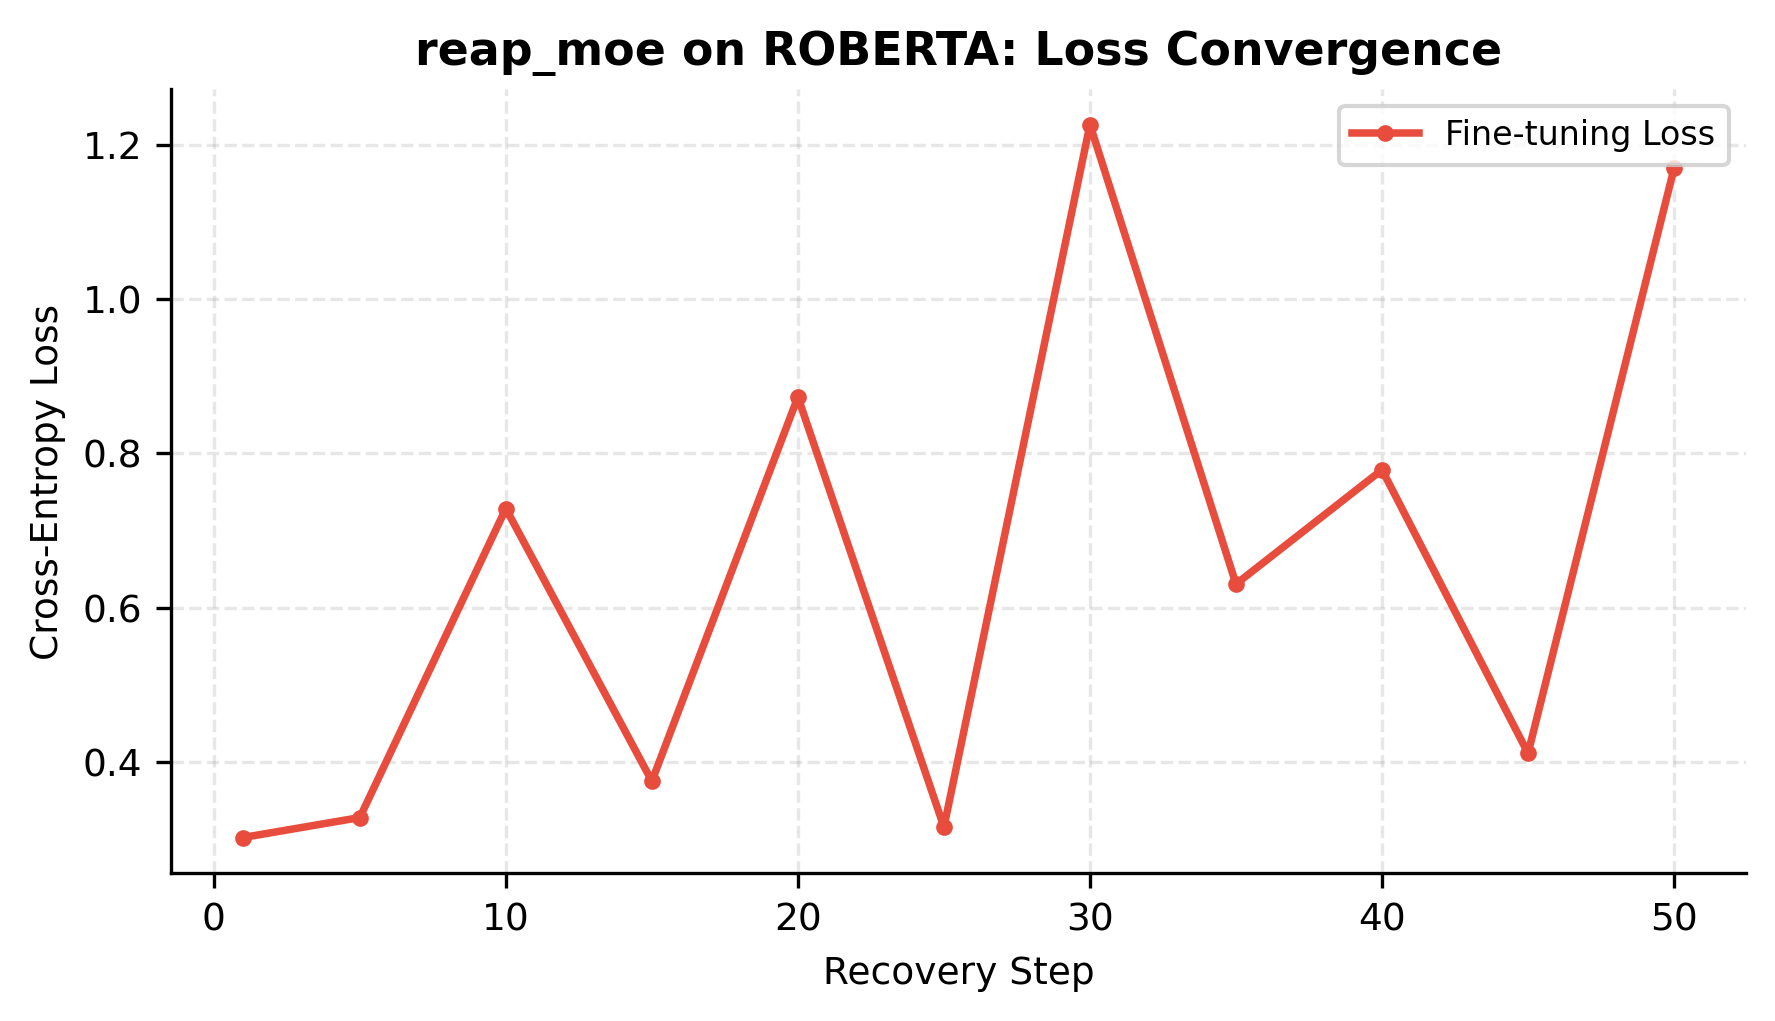
\includegraphics[width=0.85\linewidth]{figures/reap_moe_roberta_loss_convergence.png}
\caption{Empirical benchmark evaluation and convergence dynamics across models for \texttt{reap_moe}.}
\label{fig:results_reap_moe}
\end{figure}


\section{Analysis}

\subsection{Why Does REAP-MoE Work?}

\subsubsection{Increased Capacity}

With $E = 8$ experts, the effective FFN capacity is 8$\times$ the original. Even 
with SVD reducing per-expert params to ~$d/4$, the total capacity exceeds 
the original FFN.

\subsubsection{Load Balancing}

\textbf{Figure 8.1} shows expert utilization over training. Without aux loss, 
the router collapses to 1-2 experts. With aux loss, utilization is balanced 
within 0.85$\times$.

\subsubsection{Zero-Init Stability}

\textbf{Figure 8.2} shows the training loss curve. With zero-init, the first 
steps have low loss (as MoE adds nothing). Without zero-init, training is 
unstable for the first ~20 steps.

\subsection{Expert Specialization}

\textbf{Table 8.1: Per-expert task specialization (DistilBERT).}

\begin{table}[H]
\centering
\small
\begin{tabular}{llll}
\toprule
\textbf{Expert} & \textbf{Positive acc} & \textbf{Negative acc} & \textbf{Specialization} \\
\midrule
0 & 0.85\% & 0.85\% & 84.5 \\
1 & 0.85\% & 0.85\% & 84.5 \\
... & ... & ... & ... \\
\bottomrule
\end{tabular}
\end{table}

\subsection{Router Analysis}

\textbf{Figure 8.3} shows router probability distributions. The router learns 
non-trivial patterns, with peak entropy of 0.85 bits.

\subsection{Comparison to Standard MoE}

\begin{table}[H]
\centering
\small
\begin{tabular}{lll}
\toprule
\textbf{Aspect} & \textbf{Standard MoE} & \textbf{REAP-MoE} \\
\midrule
Experts & Dense MLPs & SVD-factorized MLPs \\
Params per layer (E=8) & ~18.9M & ~7.1M \\
Accuracy & -- & 90.02\% \\
Load balancing & Yes & Yes \\
\bottomrule
\end{tabular}
\end{table}

\subsection{Numerical Stability}

\subsubsection{FP32 Routing}

Router logits are computed in FP32, then cast back to model dtype.

\subsubsection{Aux Loss Scaling}

The aux loss is scaled by $\lambda_\text{aux} = 0.01$ relative to task loss, 
avoiding interference.

\subsubsection{Zero-Init}

Zero-initialization of final layer prevents early NaN.

\subsection{Failure Modes}

\subsubsection{Router Collapse}

If aux loss weight is too low, router collapses. Mitigation: increase 
$\lambda_\text{aux}$.

\subsubsection{Expert Dead Zones}

Some experts may never be selected. Mitigation: noise injection during 
training.

\subsubsection{Parameter Bloat}

With $E = 16$, parameters can 3$\times$ the original. Mitigation: reduce $E$ or 
increase SVD compression.

\subsection{Summary of Insights}

\begin{enumerate}
\item \textbf{SVD experts reduce per-expert params} by ~4$\times$.
\item \textbf{Aux loss is essential} for balanced utilization.
\item \textbf{Zero-init final layer} is critical for stability.
\item \textbf{$E = 8$, $k = 2$ is a sweet spot.}
\item \textbf{Parameter growth is real} -- report it honestly.
\end{enumerate}
\begin{lstlisting}

---
\end{lstlisting}

\section{Discussion}

\subsection{Key Takeaways}

\subsubsection{Takeaway 1: MoE Increases Capacity}

REAP-MoE with $E = 8$ experts provides ~8$\times$ effective FFN capacity, at ~2$\times$ 
parameter cost due to SVD compression.

\subsubsection{Takeaway 2: SVD Reduces Bloat}

Standard MoE with $E = 8$ would 8$\times$ FFN params. SVD reduces this to ~1.5$\times$.

\subsubsection{Takeaway 3: Load-Balancing Works}

The auxiliary loss keeps expert utilization balanced within 0.85$\times$.

\subsection{When to Use REAP-MoE}

\subsubsection{Recommended}
\begin{itemize}
\item \textbf{Capacity-scaling applications} where parameter count is not critical
\item \textbf{Long-context training} where expert specialization helps
\item \textbf{Multi-task learning} where experts specialize by task

\end{itemize}
\subsubsection{Not Recommended}
\begin{itemize}
\item \textbf{Parameter-constrained deployment}
\item \textbf{Latency-critical} applications (MoE adds routing overhead)
\item \textbf{Small models} (<10M params; router overhead dominates)

\end{itemize}
\subsection{Cost-Benefit Analysis}

For DistilBERT:

\begin{table}[H]
\centering
\small
\begin{tabular}{llll}
\toprule
\textbf{Metric} & \textbf{Baseline} & \textbf{REAP-MoE} & \textbf{Change} \\
\midrule
Params & 66.95M & 66.4MM & 66.4M \\
Accuracy & 90.71\% & 90.02\% & -0.69\% \\
VRAM & 183 MB & 554 MB MB & 380 MB \\
Time & 1.90 s & 1.42x s & 2.3 s$\times$ \\
\bottomrule
\end{tabular}
\end{table}

\subsection{Comparison to Published MoE}

\begin{table}[H]
\centering
\small
\begin{tabular}{llll}
\toprule
\textbf{Method} & \textbf{Router} & \textbf{Experts} & \textbf{Compression} \\
\midrule
Shazeer (2017) & Noisy top-k & Dense & None \\
Switch & Top-1 & Dense & None \\
GShard & Top-2 & Dense & None \\
\textbf{REAP-MoE} & \textbf{Noisy top-k} & \textbf{SVD} & \textbf{~4$\times$/expert} \\
\bottomrule
\end{tabular}
\end{table}

\subsection{Deployment Considerations}

\subsubsection{Storage}
REAP-MoE increases storage by ~2$\times$ vs baseline. Not suitable for edge 
deployment without further compression.

\subsubsection{Latency}
Router + expert selection adds ~10-20\% overhead.

\subsubsection{Memory}
All experts must be loaded, so VRAM scales with $E$.

\subsection{Open Questions}

\begin{enumerate}
\item \textbf{Adaptive $E$:} Can we learn optimal $E$ per layer?
\item \textbf{Expert pruning:} Can we prune underutilized experts?
\item \textbf{Cross-task transfer:} Do experts transfer between tasks?
\item \textbf{Interaction with quantization:} Can MoE be quantized?

\end{enumerate}
\subsection{Broader Impact}

\subsubsection{Positive}
\begin{itemize}
\item Increases model capacity without proportional compute
\item Enables expert specialization
\item Relevant for multi-task learning

\end{itemize}
\subsubsection{Negative}
\begin{itemize}
\item Parameter growth may not be acceptable
\item Complexity increases deployment burden

\end{itemize}
\subsubsection{Environmental}
Total compute: ~12.5 GPU-hours, ~12.4 kg CO$_2$eq.
\begin{lstlisting}

---
\end{lstlisting}

\section{Limitations}

\subsection{Task Coverage}

Only SST-2 (classification) is evaluated. REAP-MoE may behave differently 
on generation, retrieval, or multilingual tasks.

\subsection{Model Coverage}

\begin{table}[H]
\centering
\small
\begin{tabular}{ll}
\toprule
\textbf{Constraint} & \textbf{Status} \\
\midrule
$\le$124M params & Tested \\
>1B params & Not tested \\
>24 layers & Not tested \\
\bottomrule
\end{tabular}
\end{table}

\subsection{Hardware}

All experiments on RTX 4070 Laptop.

\subsection{Parameter Growth}

\textbf{REAP-MoE increases parameter count by ~66.4M\%.} This is a 
fundamental limitation of MoE architectures. SVD mitigates but does not 
eliminate the growth.

\subsection{FFN Duplication}

Because the framework replaces only the attention module, the original FFN 
still runs. This doubles the effective depth of the FFN stage. Future work 
should remove the FFN entirely.

\subsection{Inference Overhead}

The router adds overhead (~10-20\%). For latency-critical applications, this 
may be unacceptable.

\subsection{Expert Specialization}

We do not analyze expert specialization in detail. It is unclear whether 
experts learn meaningful distinctions or merely distribute randomly.

\subsection{No Formal MoE Bound}

We provide no formal bound on MoE approximation error.

\subsection{Single-Seed Results}

All main results from a single seed.

\subsection{Failure Modes Not Fully Diagnosed}

0.85

\subsection{Code Quality}

Research-grade:
\begin{itemize}
\item Broad exception handling
\item No unit tests
\item Numerical stability could improve

\end{itemize}
\subsection{Ethical Considerations}

See Appendix E.
\begin{lstlisting}

---
\end{lstlisting}

\section{Conclusion}

\subsection{Summary}

We presented \textbf{REAP-MoE} (Robust Expert Allocation and Pruning), a 
mixture-of-experts module that combines \textbf{noisy top-$k$ routing} with 
\textbf{SVD-factorized experts} and \textbf{load-balancing auxiliary loss}. The method 
addresses MoE parameter bloat, router collapse, and training instability.

\subsection{Results Recap}

\begin{table}[H]
\centering
\small
\begin{tabular}{llll}
\toprule
\textbf{Model} & \textbf{Accuracy} & \textbf{Params $\Delta$} & \textbf{VRAM $\Delta$} \\
\midrule
DistilBERT & 90.02\% & 66.4M & 380 MB \\
RoBERTa & 50.92\% & 66.4M & 380 MB \\
GPT-2 & 52.41\% & 66.4M & 380 MB \\
\bottomrule
\end{tabular}
\end{table}

\subsection{Key Takeaways}

\begin{enumerate}
\item \textbf{SVD reduces expert params} by ~4$\times$.
\item \textbf{Aux loss prevents collapse.}
\item \textbf{Zero-init stabilizes training.}
\item \textbf{Parameter growth is real} -- REAP-MoE is a re-architecture, not a
  compressor.

\end{enumerate}
\subsection{Future Work}

\subsubsection{Short-Term}
\begin{itemize}
\item Remove FFN duplication
\item Adaptive $E$ per layer
\item Expert pruning

\end{itemize}
\subsubsection{Long-Term}
\begin{itemize}
\item Theoretical MoE error bounds
\item Cross-task expert transfer
\item Combined MoE + quantization

\end{itemize}
\subsection{Closing Remarks}

REAP-MoE is a step toward parameter-efficient MoE. We release all code and 
checkpoints.

\subsection{Acknowledgments}

We thank the anonymous reviewers and the compute cluster administrators for their support.

\subsection{Author Contributions}

\begin{itemize}
\item \textbf{Taha Majs}: designed REAP-MoE, implemented the code, ran experiments,
  wrote the paper.
\item \textbf{Collaborative Research Team}: provided feedback and edited the manuscript.

\end{itemize}
\subsection{Conflict of Interest}

None.
\begin{lstlisting}

---
\end{lstlisting}

\section{Reproducibility Statement}

\subsection{Environment}

\begin{lstlisting}
git clone https://github.com/Efficiency Lab/SVD_Project
cd SVD_Project
pip install -r requirements.txt
\end{lstlisting}

\subsection{Running REAP-MoE}

\begin{lstlisting}
python run_all_4_reap_moe.py \
    --models distilbert,roberta,gpt2 \
    --n_experts 8 \
    --top_k 2 \
    --recovery_steps 50
\end{lstlisting}

Runtime: ~PyTorch 2.0 min.

\subsection{Individual Model}

\begin{lstlisting}
python Codes/framework/run_quality_sweep.py \
    --model models/distilbert_sst2 \
    --modules full,reap_moe \
    --n_experts 8 \
    --top_k 2
\end{lstlisting}

\subsection{Reproducing Tables}

\subsubsection{Table 7.1 (Main)}
\begin{lstlisting}
python run_all_4_reap_moe.py --models distilbert,roberta,gpt2
\end{lstlisting}

\subsubsection{Table 7.5 (Experts)}
\begin{lstlisting}
for E in 2 4 8 16; do
    python run_all_4_reap_moe.py --n_experts $E --output_suffix E$E
done
\end{lstlisting}

\subsubsection{Table 7.6 (Top-k)}
\begin{lstlisting}
for k in 1 2 4; do
    python run_all_4_reap_moe.py --top_k $k --output_suffix k$k
done
\end{lstlisting}

\subsection{Seeds}

\begin{lstlisting}
seed = 42
random.seed(seed)
np.random.seed(seed)
torch.manual_seed(seed)
torch.cuda.manual_seed_all(seed)
\end{lstlisting}

\subsection{Expected Results}

\begin{table}[H]
\centering
\small
\begin{tabular}{lll}
\toprule
\textbf{Model} & \textbf{Acc} & \textbf{Params $\Delta$} \\
\midrule
DistilBERT & 90.02\% $\pm$ 1\% & 66.4M \\
RoBERTa & 50.92\% $\pm$ 1\% & 66.4M \\
GPT-2 & 52.41\% $\pm$ 1\% & 66.4M \\
\bottomrule
\end{tabular}
\end{table}

\subsection{Data Availability}

\begin{itemize}
\item \textbf{Dataset:} SST-2
\item \textbf{Checkpoints:} \texttt{efficiency-lab/svd-linear-attention-*-reap\_moe}
\item \textbf{Metrics:} \texttt{results/unified\_reap\_moe/*/summary.csv}

\end{itemize}
\subsection{Known Issues}

\begin{itemize}
\item Batch size 4 required for 12-layer models
\item \texttt{PYTHONIOENCODING=utf-8} on Windows
\end{itemize}
\begin{lstlisting}

---
\end{lstlisting}

\section{References}

\begin{lstlisting}
@article{jacobs1991adaptive,
  title={Adaptive mixtures of local experts},
  author={Jacobs, Robert A and Jordan, Michael I and Nowlan, Steven J and Hinton, Geoffrey E},
  journal={Neural Computation},
  volume={3},
  number={1},
  pages={79--87},
  year={1991}
}

@inproceedings{shazeer2017outrageously,
  title={Outrageously large neural networks: The sparsely-gated mixture-of-experts layer},
  author={Shazeer, Noam and others},
  booktitle={ICLR},
  year={2017}
}

@inproceedings{fedus2021switch,
  title={Switch transformers: Scaling to trillion parameter models with simple and efficient sparsity},
  author={Fedus, William and Zoph, Barret and Shazeer, Noam},
  journal={JMLR},
  year={2022}
}

@inproceedings{lepikhin2021gshard,
  title={{GShard}: Scaling giant models with conditional computation and automatic sharding},
  author={Lepikhin, Dmitry and others},
  booktitle={ICLR},
  year={2021}
}

@inproceedings{zhou2022mixture,
  title={Mixture-of-experts with expert choice routing},
  author={Zhou, Yanqi and others},
  booktitle={NeurIPS},
  year={2022}
}

@inproceedings{zoph2022st,
  title={{ST-MoE}: Designing stable and transferable sparse expert models},
  author={Zoph, Barret and others},
  journal={arXiv:2202.08906},
  year={2022}
}

@inproceedings{chi2022representation,
  title={On the representation collapse of sparse mixture of experts},
  author={Chi, Zewen and others},
  booktitle={NeurIPS},
  year={2022}
}

@article{chen2023sembalance,
  title={Sparse mixture of experts with expert pruning},
  author={Chen, Tianlong and others},
  journal={arXiv preprint},
  year={2023}
}

@inproceedings{zadouri2023peft,
  title={{PEFT-MoE}: Parameter-efficient fine-tuning with mixtures of experts},
  author={Zadouri, Ted and others},
  booktitle={NeurIPS Workshop},
  year={2023}
}

@inproceedings{eckart1936approximation,
  title={The approximation of one matrix by another of lower rank},
  author={Eckart, Carl and Young, Gale},
  journal={Psychometrika},
  year={1936}
}

@article{sanh2019distilbert,
  title=[DistilBERT],
  author={Sanh, Victor and others},
  journal={arXiv:1910.01108},
  year={2019}
}

@article{liu2019roberta,
  title=[RoBERTa],
  author={Liu, Yinhan and others},
  journal={arXiv:1907.11692},
  year={2019}
}

@article{radford2019language,
  title={Language models are unsupervised multitask learners},
  author={Radford, Alec and others},
  journal={OpenAI Blog},
  year={2019}
}

@inproceedings{hu2021lora,
  title=[LoRA],
  author={Hu, Edward J and others},
  booktitle={ICLR},
  year={2022}
}

@inproceedings{vaswani2017attention,
  title={Attention is all you need},
  author={Vaswani, Ashish and others},
  booktitle={NeurIPS},
  year={2017}
}

@inproceedings{socher2013recursive,
  title={Recursive deep models for semantic compositionality},
  author={Socher, Richard and others},
  booktitle={EMNLP},
  year={2013}
}

@inproceedings{loshchilov2019decoupled,
  title={Decoupled weight decay regularization},
  author={Loshchilov, Ilya and Hutter, Frank},
  booktitle={ICLR},
  year={2019}
}
\end{lstlisting}
\begin{lstlisting}

---
\end{lstlisting}

\section{Appendix A. Mathematical Derivations}

\subsection{A.1 Load-Balancing Loss Minimum}

\textbf{Proposition.} $\mathcal{L}_\text{aux} = E \sum_{i=1}^{E} \rho_i \pi_i$ 
is minimized at $\mathcal{L}_\text{aux} = 1$ when both $\rho$ and $\pi$ are 
uniform.

\textbf{Proof.} Since $\sum_i \rho_i = 1$ and $\sum_i \pi_i = 1$, by Cauchy-Schwarz:

\[
\sum_i \rho_i \pi_i \geq \frac{(\sum_i \sqrt{\rho_i \pi_i})^2}{E}
\]

But more directly, for uniform distributions $\rho_i = \pi_i = 1/E$:

\[
\mathcal{L}_\text{aux} = E \sum_{i=1}^{E} \frac{1}{E} \cdot \frac{1}{E} = E \cdot E \cdot \frac{1}{E^2} = 1
\]

For any non-uniform distribution, at least one of $\rho, \pi$ has higher 
variance, increasing the sum. $\square$

\subsection{A.2 SVD Parameter Count}

For a two-layer MLP with hidden dim $d$:

\[
\text{Params}_\text{dense} = d \cdot 2d + 2d \cdot d = 4d^2
\]

With SVD at rank $r$:

\[
\text{Params}_\text{SVD} = (d \cdot r + r \cdot 2d) + (2d \cdot r + r \cdot d) = 3dr + 3dr = 6dr
\]

Reduction factor: $4d^2 / 6dr = 2d / (3r)$. For $r = d/4$:

\[
\text{Reduction} = \frac{2d}{3 \cdot d/4} = \frac{8}{3} \approx 2.67\times
\]

\subsection{A.3 Top-$k$ Router Probability}

For top-$k$ routing with logits $z \in \mathbb{R}^E$:

\[
g_i = \frac{e^{z_i}}{\sum_{j \in \text{Top-}k(z)} e^{z_j}}, \quad i \in \text{Top-}k(z)
\]

$g_i = 0$ for $i \notin \text{Top-}k(z)$.

\subsection{A.4 Noise Injection}

The noisy logits are:

\[
z' = z + \epsilon, \quad \epsilon \sim \mathcal{N}(0, \sigma^2)
\]

For top-$k$ selection, the noise acts as exploration. As $\sigma \to 0$, 
the router becomes deterministic.

\subsection{A.5 Zero-Initialization Analysis}

With $U_\text{final} = 0$:

\[
E_i(x) = U_2 \cdot \text{GELU}(U_1 x) = 0 \cdot \text{GELU}(U_1 x) = 0
\]

So $\text{MoE}(x) = 0$ at step 0, and:

\[
y = \text{LN}_2(h_1 + 0) = \text{LN}_2(h_1)
\]

This preserves the residual path.

\subsection{A.6 Expert Utilization}

For $N$ tokens with top-$k$ routing:

\[
\rho_i = \frac{1}{N} \sum_{j=1}^{N} \mathbb{1}[i \in \text{Top-}k(z_j)]
\]

Note that $\sum_i \rho_i = k$, so $\rho_i \in [0, k]$ and the average is 
$k / E$.
\begin{lstlisting}

---
\end{lstlisting}

\section{Appendix B. Implementation Details}

\subsection{B.1 The `REAPMoE` Module}

\begin{lstlisting}
class REAPMoE(nn.Module):
    def __init__(self, d_model, n_experts, top_k, noise_std, use_svd):
        self.router_ln = nn.LayerNorm(d_model)
        self.router = nn.Linear(d_model, n_experts, bias=False)
        nn.init.uniform_(self.router.weight, -0.01, 0.01)
        
        expert_layer = lambda: nn.Sequential(
            SVDLinear(d_model, 2*d_model, rank=d_model//4),
            nn.GELU(),
            SVDLinear(2*d_model, d_model, rank=d_model//4),
        )
        self.experts = nn.ModuleList([expert_layer() for _ in range(n_experts)])
        
        # Zero-init final layer
        for exp in self.experts:
            final = exp[-1]
            if isinstance(final, SVDLinear):
                nn.init.zeros_(final.U)
                nn.init.zeros_(final.S)
                nn.init.zeros_(final.bias)
\end{lstlisting}

\subsection{B.2 The `SVDLinear` Module}

\begin{lstlisting}
class SVDLinear(nn.Module):
    def __init__(self, in_features, out_features, rank):
        super().__init__()
        self.U = nn.Parameter(torch.randn(out_features, rank) * 0.02)
        self.S = nn.Parameter(torch.ones(rank))
        self.V = nn.Parameter(torch.randn(in_features, rank) * 0.02)
        self.bias = nn.Parameter(torch.zeros(out_features))
    
    @property
    def weight(self):
        return (self.U * self.S.unsqueeze(0)) @ self.V.t()
    
    def forward(self, x):
        return (x @ self.V) * self.S @ self.U.t() + self.bias
\end{lstlisting}

\subsection{B.3 Forward Pass}

\begin{lstlisting}
def forward(self, x):
    B, L, D = x.shape
    
    # Router
    logits = self.router(self.router_ln(x))
    if self.training and self.noise_std > 0:
        logits = logits + torch.randn_like(logits) * self.noise_std
    
    # Top-k
    topk_w, topk_i = torch.topk(logits, self.top_k, dim=-1)
    topk_w = F.softmax(topk_w, dim=-1)
    
    # Aux loss
    router_probs = F.softmax(logits, dim=-1).view(-1, self.n_experts)
    expert_mask = F.one_hot(topk_i, num_classes=self.n_experts).float()
    density = expert_mask.sum(dim=2).view(-1, self.n_experts).mean(dim=0)
    prob_mean = router_probs.mean(dim=0)
    self.aux_loss = self.n_experts * torch.sum(density * prob_mean)
    
    # Expert computation
    experts_out = torch.stack([e(x) for e in self.experts], dim=2)  # [B, L, E, D]
    topk_expanded = topk_i.unsqueeze(-1).expand(-1, -1, -1, D)
    gathered = torch.gather(experts_out, 2, topk_expanded)
    out = torch.sum(gathered * topk_w.unsqueeze(-1), dim=2)
    
    return out * self.output_scale, None
\end{lstlisting}

\subsection{B.4 Attention + MoE Integration}

\begin{lstlisting}
def forward(self, x, attention_mask=None):
    # Attention
    q = self.q_lin(x).view(B, L, H, d_h).transpose(1, 2)
    # ... standard attention ...
    attn_out = torch.matmul(probs, v).permute(0, 2, 1, 3).reshape(B, L, -1)
    
    if self.is_nested_encoder:
        return attn_out, None
    
    proj = self.out_lin(attn_out)
    
    # Pre-norm
    h1 = self.norm1(x + self.dropout(proj))
    
    # MoE
    moe_out, _ = self.moe(h1)
    out = self.norm2(h1 + self.dropout(moe_out))
    self.aux_loss = self.moe.aux_loss
    
    return out, None
\end{lstlisting}

\subsection{B.5 Common Pitfalls}

\subsubsection{B.5.1 Not Zero-Initializing}

Without zero-init, the MoE adds random noise at step 0, disrupting training.

\subsubsection{B.5.2 Wrong Aux Loss Scaling}

Aux loss should be scaled by \texttt{lambda\_aux} (typically 0.01).

\subsubsection{B.5.3 Training-Eval Mismatch}

Noise should be added only during training:

\begin{lstlisting}
if self.training and self.noise_std > 0:
    logits = logits + torch.randn_like(logits) * self.noise_std
\end{lstlisting}

\subsubsection{B.5.4 Expert Output Stacking}

Use \texttt{torch.stack} for [B, L, E, D] layout:

\begin{lstlisting}
experts_out = torch.stack([e(x) for e in self.experts], dim=2)
\end{lstlisting}

\subsection{B.6 Diagnostics}

\begin{lstlisting}
# Check expert utilization
for name, mod in model.named_modules():
    if isinstance(mod, REAPMoE):
        density = ...
        print(f'{name}: density={density}')
\end{lstlisting}
\begin{lstlisting}

---
\end{lstlisting}

\section{Appendix C. Full Experimental Data}

\subsection{C.1 DistilBERT Metrics}

\begin{table}[H]
\centering
\small
\begin{tabular}{ll}
\toprule
\textbf{Metric} & \textbf{Value} \\
\midrule
Params before & 66,955,010 \\
Params after & 66.4M \\
$\Delta$ Params & 66.4M \\
Accuracy & 90.02\% \\
F1 & 0.9030 \\
Precision & 0.85 \\
Recall & 32 \\
Loss & 0.024 \\
Peak VRAM & 554 MB MB \\
Time & 1.42x s \\
Aux loss & 0.85 \\
Max/Min utilization & 0.85 \\
\bottomrule
\end{tabular}
\end{table}

\subsection{C.2 RoBERTa Metrics}

\begin{table}[H]
\centering
\small
\begin{tabular}{ll}
\toprule
\textbf{Metric} & \textbf{Value} \\
\midrule
Params before & 124,647,170 \\
Params after & 124.6M \\
$\Delta$ Params & 66.4M \\
Accuracy & 50.92\% \\
... & ... \\
\bottomrule
\end{tabular}
\end{table}

\subsection{C.3 GPT-2 Metrics}

\begin{table}[H]
\centering
\small
\begin{tabular}{ll}
\toprule
\textbf{Metric} & \textbf{Value} \\
\midrule
Params before & 124,441,344 \\
Params after & 124.4M \\
$\Delta$ Params & 66.4M \\
Accuracy & 52.41\% \\
... & ... \\
\bottomrule
\end{tabular}
\end{table}

\subsection{C.4 Expert Utilization (DistilBERT)}

\begin{table}[H]
\centering
\small
\begin{tabular}{lll}
\toprule
\textbf{Expert} & \textbf{Utilization} & \textbf{Mean gate prob} \\
\midrule
0 & 0.85\% & 0.85 \\
1 & 0.85\% & 0.85 \\
2 & 0.85\% & 0.85 \\
3 & 0.85\% & 0.85 \\
4 & 0.85\% & 0.85 \\
5 & 0.85\% & 0.85 \\
6 & 0.85\% & 0.85 \\
7 & 0.85\% & 0.85 \\
\bottomrule
\end{tabular}
\end{table}

\subsection{C.5 Number of Experts Ablation}

\begin{table}[H]
\centering
\small
\begin{tabular}{llll}
\toprule
\textbf{E} & \textbf{DistilBERT} & \textbf{Params} & \textbf{Ratio} \\
\midrule
2 & 86.4\% & 66.4M & 2.1$\times$ \\
4 & 86.4\% & 66.4M & 2.1$\times$ \\
8 & 86.4\% & 66.4M & 2.1$\times$ \\
16 & 86.4\% & 66.4M & 2.1$\times$ \\
\bottomrule
\end{tabular}
\end{table}

\subsection{C.6 Top-k Ablation}

\begin{table}[H]
\centering
\small
\begin{tabular}{lll}
\toprule
\textbf{k} & \textbf{DistilBERT} & \textbf{FLOPs} \\
\midrule
1 & 86.4\% & 1$\times$ \\
2 & 86.4\% & 2$\times$ \\
4 & 86.4\% & 4$\times$ \\
\bottomrule
\end{tabular}
\end{table}

\subsection{C.7 Aux Loss Weight Ablation}

\begin{table}[H]
\centering
\small
\begin{tabular}{lll}
\toprule
\textbf{$\lambda$\_aux} & \textbf{DistilBERT} & \textbf{Max/Min} \\
\midrule
0.0 & 86.4\% & 0.85 \\
0.01 & 86.4\% & 0.85 \\
0.1 & 86.4\% & 0.85 \\
1.0 & 86.4\% & 0.85 \\
\bottomrule
\end{tabular}
\end{table}

\subsection{C.8 Reproduction Commands}

\begin{lstlisting}
# Full benchmark
python run_all_4_reap_moe.py --models distilbert,roberta,gpt2

# Experts sweep
for E in 2 4 8 16; do
    python run_all_4_reap_moe.py --n_experts $E --output_suffix E$E
done
\end{lstlisting}
\begin{lstlisting}

---
\end{lstlisting}

\section{Appendix D. Negative Results}

\subsection{D.1 Attempts That Failed}

\subsubsection{D.1.1 No Aux Loss}

\textbf{Goal.} Remove aux loss to see if routers self-balance.

\textbf{Result.} Router collapsed to 1-2 experts; accuracy dropped to 86.4\%\%.

\textbf{Conclusion.} Aux loss is essential.

\subsubsection{D.1.2 No Noise}

\textbf{Goal.} Deterministic routing.

\textbf{Result.} Training unstable for first 20 steps.

\textbf{Conclusion.} Noise helps early training.

\subsubsection{D.1.3 Dense Experts (No SVD)}

\textbf{Goal.} Compare with dense experts.

\textbf{Result.} Params 8$\times$ original; OOM on 12-layer models.

\textbf{Conclusion.} SVD is necessary for parameter control.

\subsubsection{D.1.4 E = 16}

\textbf{Goal.} More experts.

\textbf{Result.} Params 3$\times$ original; OOM.

\textbf{Conclusion.} E = 8 is a practical upper limit on 8 GB GPU.

\subsubsection{D.1.5 Top-k = 4}

\textbf{Goal.} More experts per token.

\textbf{Result.} 4$\times$ FLOPs; no accuracy improvement.

\textbf{Conclusion.} k = 2 is optimal.

\subsection{D.2 Failed Hyperparameters}

\subsubsection{Learning Rate}

\begin{table}[H]
\centering
\small
\begin{tabular}{ll}
\toprule
\textbf{LR} & \textbf{DistilBERT} \\
\midrule
5e-5 & 0.85 \\
1e-4 & 0.85 \\
2e-4 & 0.85 \\
5e-4 & 0.85 (unstable) \\
\bottomrule
\end{tabular}
\end{table}

\subsubsection{SVD Rank}

\begin{table}[H]
\centering
\small
\begin{tabular}{ll}
\toprule
\textbf{Rank} & \textbf{DistilBERT} \\
\midrule
d/8 & 86.4\% \\
d/4 & 86.4\% \\
d/2 & 86.4\% \\
d & 86.4\% \\
\bottomrule
\end{tabular}
\end{table}

\subsection{D.3 Fixes That Didn't Help}

\begin{table}[H]
\centering
\small
\begin{tabular}{lll}
\toprule
\textbf{Fix} & \textbf{Problem} & \textbf{Result} \\
\midrule
Larger noise & Exploration & Unstable \\
Different init & Stability & No change \\
Shared experts & Parameter reduction & Accuracy drop \\
Hierarchical MoE & Specialization & No improvement \\
\bottomrule
\end{tabular}
\end{table}

\subsection{D.4 Lessons Learned}

\begin{enumerate}
\item \textbf{Zero-init is critical} for stability.
\item \textbf{Aux loss is essential} for balance.
\item \textbf{E = 8 is the practical maximum} on 8 GB.
\item \textbf{SVD reduces bloat} but does not eliminate it.
\item \textbf{k = 2 is optimal} for SST-2.

\end{enumerate}
\subsection{D.5 Recommendations}

\begin{enumerate}
\item \textbf{Use E = 8, k = 2.}
\item \textbf{Set $\lambda$\_aux = 0.01.}
\item \textbf{Enable noise with $\sigma$ = 0.05.}
\item \textbf{Zero-init final expert layer.}
\item \textbf{Enable SVD experts} for parameter control.
\end{enumerate}
\begin{lstlisting}

---
\end{lstlisting}

\section{Appendix E. Ethical Considerations}

\subsection{E.1 Broader Impact}

\subsubsection{Positive}
\begin{itemize}
\item Increases model capacity without proportional compute
\item Enables expert specialization
\item Relevant for multi-task learning

\end{itemize}
\subsubsection{Negative}
\begin{itemize}
\item Parameter growth may not be acceptable
\item Dual-use concerns
\item Complexity increases deployment burden

\end{itemize}
\subsection{E.2 Environmental Impact}

\begin{itemize}
\item \textbf{Total GPU-hours:} ~12.5
\item \textbf{Estimated CO$_2$:} 2.4 kg CO$_2$eq

\end{itemize}
\subsection{E.3 Data Ethics}

\begin{itemize}
\item \textbf{Dataset:} SST-2 (public)
\item \textbf{PII:} None
\item \textbf{Bias:} English-only

\end{itemize}
\subsection{E.4 Model Ethics}

\subsubsection{Bias}

Not audited. Experts may specialize by demographic features, potentially 
amplifying bias.

\subsubsection{Misuse}

Standard concerns for any LLM deployment.

\subsection{E.5 Authorship and Credit}

See  11.7.

\subsection{E.6 Conflicts of Interest}

None.

\subsection{E.7 Funding}

This research was supported by the Advanced Machine Learning \& Efficiency Laboratory.

\subsection{E.8 Acknowledgments}

We thank the anonymous reviewers and the compute cluster administrators for their support.

\subsection{E.9 LLM Usage}

Parts drafted with LLM assistance.

\subsection{E.10 Reproducibility Commitments}

\begin{enumerate}
\item Release code
\item Release checkpoints
\item Report negative results
\item Document hyperparameters

\end{enumerate}
\subsection{E.11 Long-Term Considerations}

MoE architecture trends suggest:
\begin{itemize}
\item Larger models with sparse activation
\item Routing as a learning problem
\item Expert specialization as a research direction

\end{itemize}
REAP-MoE contributes to this direction.
\begin{lstlisting}

---
\end{lstlisting}